\documentclass{article}\usepackage[]{graphicx}\usepackage[]{color}
%% maxwidth is the original width if it is less than linewidth
%% otherwise use linewidth (to make sure the graphics do not exceed the margin)
\makeatletter
\def\maxwidth{ %
  \ifdim\Gin@nat@width>\linewidth
    \linewidth
  \else
    \Gin@nat@width
  \fi
}
\makeatother

\definecolor{fgcolor}{rgb}{0.345, 0.345, 0.345}
\newcommand{\hlnum}[1]{\textcolor[rgb]{0.686,0.059,0.569}{#1}}%
\newcommand{\hlstr}[1]{\textcolor[rgb]{0.192,0.494,0.8}{#1}}%
\newcommand{\hlcom}[1]{\textcolor[rgb]{0.678,0.584,0.686}{\textit{#1}}}%
\newcommand{\hlopt}[1]{\textcolor[rgb]{0,0,0}{#1}}%
\newcommand{\hlstd}[1]{\textcolor[rgb]{0.345,0.345,0.345}{#1}}%
\newcommand{\hlkwa}[1]{\textcolor[rgb]{0.161,0.373,0.58}{\textbf{#1}}}%
\newcommand{\hlkwb}[1]{\textcolor[rgb]{0.69,0.353,0.396}{#1}}%
\newcommand{\hlkwc}[1]{\textcolor[rgb]{0.333,0.667,0.333}{#1}}%
\newcommand{\hlkwd}[1]{\textcolor[rgb]{0.737,0.353,0.396}{\textbf{#1}}}%

\usepackage{framed}
\makeatletter
\newenvironment{kframe}{%
 \def\at@end@of@kframe{}%
 \ifinner\ifhmode%
  \def\at@end@of@kframe{\end{minipage}}%
  \begin{minipage}{\columnwidth}%
 \fi\fi%
 \def\FrameCommand##1{\hskip\@totalleftmargin \hskip-\fboxsep
 \colorbox{shadecolor}{##1}\hskip-\fboxsep
     % There is no \\@totalrightmargin, so:
     \hskip-\linewidth \hskip-\@totalleftmargin \hskip\columnwidth}%
 \MakeFramed {\advance\hsize-\width
   \@totalleftmargin\z@ \linewidth\hsize
   \@setminipage}}%
 {\par\unskip\endMakeFramed%
 \at@end@of@kframe}
\makeatother

\definecolor{shadecolor}{rgb}{.97, .97, .97}
\definecolor{messagecolor}{rgb}{0, 0, 0}
\definecolor{warningcolor}{rgb}{1, 0, 1}
\definecolor{errorcolor}{rgb}{1, 0, 0}
\newenvironment{knitrout}{}{} % an empty environment to be redefined in TeX

\usepackage{alltt}

%\VignetteIndexEntry{hutchinhillproject}
\IfFileExists{upquote.sty}{\usepackage{upquote}}{}
\begin{document}

\title{What is the Average Age of the Williams College Faculty?}
\author{Daishiro Nishida '18}
\maketitle

This paper investigates the average age of the Williams College faculty. The first section calculates the
mean age of the faculty, along with other simple data such as the oldest and youngest members of the faculty.
The second section investigates how the average age varies among different departments and different
divisions. The third section explores how the completion of terminal degrees influenced the age of the
faculty.\\

\section{Mean Age of Faculty}

\subsection{Assembling the Data}
The data was collected from the Williams College Bulletin from the year 2013-14, which was found on the
website of the Registrar's Office. The data was taken from the year 2013-14 since the bulletin for the
latest calendar year, 2014-15, did not include the necessary information.\\

The information collected were the names of all professors, their departments, the year they received their
BA, and the year they received their last degree. Any professors who did not provide all of the above
information were omitted. From these data their age and the division they belong to were inferred.
All of the data were entered manually by the author.
The full data can be found in the /data folder in the package.\\

Several assumptions were made in clarifying ambiguous cases. All professors belonging to more than one
department were classified into the one mentioned first in the document. Professors belonging to departments
with only one or two professors who also taught courses in other departments were classified into departments
with more professors. This was done to make sure that each department had a sufficient number of professors
to conduct an accurate comparison among departments. Some exceptions are the Comparative Literature department
with two professors, and the Marine Sciences department with one professor, both of which were kept in the analysis as the professors could not be classified into other departments. And finally, professors of French,
Spanish, and Italian were all grouped as Romance Languages professors, since some professors were only
indicated as such and their specific language of specialty could not be determined.

\subsection{Calculating the Mean Age}
The age of the professor was calculated with the assumption that all professors received their BA at the
age of 22. Although this is clearly an underestimation, data on the average age of college students receiving
their BA could not be obtained, so this was the only reasonable assumption possible. The mean age was
calculated as of the year 2014 in order to gain an estimate of the average age at the time; the assumption
is that older professors retire and younger professors come in every year, keeping the average age consistent.
Hence the equation used to calculate the average age is $2014 - $gradyear$ + 22$, where gradyear refers to
the year the professor received his/her BA.\\

Applying this equation to all professors, and finding the mean (and the standard deviation) of the results
yields the estimated mean age of all professors at Williams College.

\begin{knitrout}
\definecolor{shadecolor}{rgb}{0.969, 0.969, 0.969}\color{fgcolor}\begin{kframe}
\begin{verbatim}
## Mean =  49.02558 
## Standard Deviation =  12.1558
\end{verbatim}
\end{kframe}
\end{knitrout}

Thus the average age of the Williams College faculty is 49.0 years, with a standard deviation of 12 years.

\subsection{Finding the Oldest and the Youngest Professors}

Now that the data is assembled, the oldest and the youngest professors can also be determined.
This can be done by arranging the data from the oldest to youngest, and looking at the top and the bottom
of the table. \\

Here is the top of the table.\\

\begin{knitrout}
\definecolor{shadecolor}{rgb}{0.969, 0.969, 0.969}\color{fgcolor}
\begin{tabular}{l|l|r|r}
\hline
name & department & year\_of\_BA & ages\\
\hline
Donald de B. Beaver & History & 1958 & 78\\
\hline
Charles B. Dew & History & 1958 & 78\\
\hline
Eugene J. Johnson III & Art & 1959 & 77\\
\hline
Marek Demianski & Astronomy & 1962 & 74\\
\hline
Anthony J. Nicastro & Romance Languages & 1962 & 74\\
\hline
\end{tabular}


\end{knitrout}
\hfill
\\
From this it can be seen that the oldest members of the faculty are Professor Donald de B. Beaver and Professor Charles B. Dew, both in the History Department. They received their BA in the year 1958 and thus their estimated age is 78 years.\\

Now here is the bottom of the table.\\

\begin{knitrout}
\definecolor{shadecolor}{rgb}{0.969, 0.969, 0.969}\color{fgcolor}
\begin{tabular}{l|l|r|r}
\hline
name & department & year\_of\_BA & ages\\
\hline
Kevin A. Escudero & Latina/o Studies & 2009 & 27\\
\hline
Marcela Romero & Romance Languages & 2009 & 27\\
\hline
Scott D. Honecker & Physical Education & 2010 & 26\\
\hline
Qing Wang & Statistics & 2010 & 26\\
\hline
Sarah A. Mirseydi & Art & 2011 & 25\\
\hline
\end{tabular}


\end{knitrout}
\hfill
\\
The youngest member of the faculty is Professor Sarah A. Mirseydi in the Art Department, who received her BA in the year 2011 and is estimated to be 25 years old.\\

\section{Comparison among Departments and Divisions}

In this section ages among different departments and divisions will be analysed through graphical
representations of the data. Firstly the age histogram of all professors can be used to examine how the
age distribution depends on the division. The division of each professor was inferred by the author,
according to their departments. The three divisions are I: Languages and the Arts, II: Social Studies, and
III: Science and Mathematics. Professors of Physical Education was classified as "PE", since they do not
belong to the three divisions.\\

Here is the histogram showing the age distribution in different divisions.

\begin{knitrout}
\definecolor{shadecolor}{rgb}{0.969, 0.969, 0.969}\color{fgcolor}\begin{figure}[h]
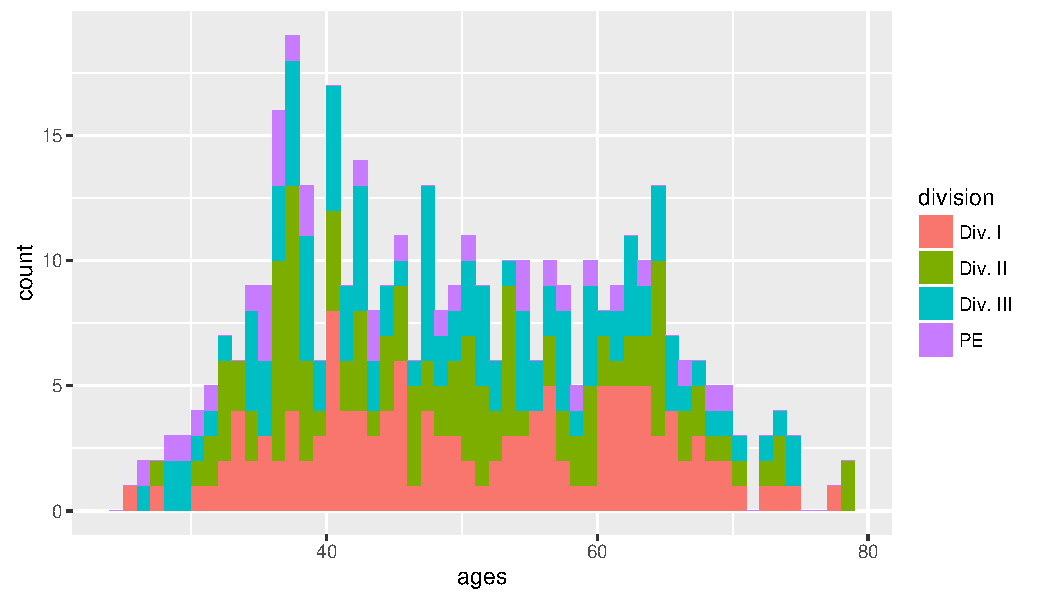
\includegraphics[width=\maxwidth]{figure/unnamed-chunk-4-1} \caption[Histogram of age distribution]{Histogram of age distribution}\label{fig:unnamed-chunk-4}
\end{figure}


\end{knitrout}

It appears that Division II and Division III have more younger professors, while in Division I the age is
distributed very evenly. As expected, Physical Education professors also seem to be younger than average, with
no professor being over 70 years of age. \\

The mean age of each division can be calculated.

\begin{knitrout}
\definecolor{shadecolor}{rgb}{0.969, 0.969, 0.969}\color{fgcolor}\begin{kframe}
\begin{verbatim}
## Div.I Mean =  50.45038 
## Div.II Mean =  48.86207 
## Div.III Mean =  48.67568 
## PE Mean =  45.12121
\end{verbatim}
\end{kframe}
\end{knitrout}

This confirms that on average, PE professors are youngest, Division I professors are oldest, and Division
II and Division III professors are somewhere in between.\\

The age distributions in each department can also be examined.

\begin{knitrout}
\definecolor{shadecolor}{rgb}{0.969, 0.969, 0.969}\color{fgcolor}\begin{figure}[h]
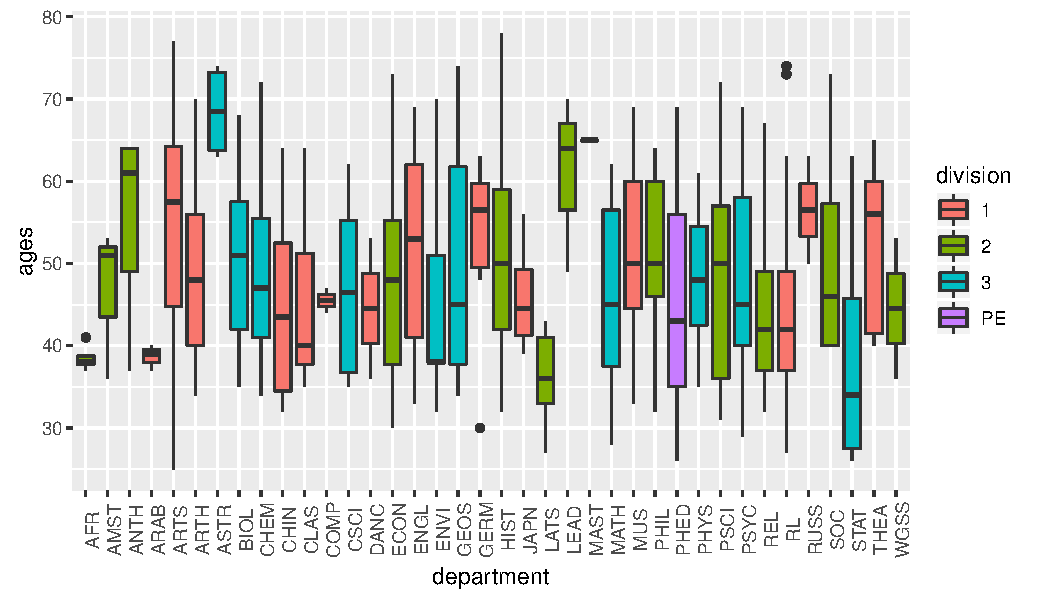
\includegraphics[width=\maxwidth]{figure/unnamed-chunk-6-1} \caption[Age distribution in each department]{Age distribution in each department}\label{fig:unnamed-chunk-6}
\end{figure}


\end{knitrout}

Four departments stand out for having a low mean age: Africana Studies, Arabic, Latina/o studies and
Statistics. Two departments that are significantly older than others are Astronomy (Division III) and
Leadership Studies (Division II). This is interesting considering Division III and Division II appeared
to be younger than Division I. However the two departments may not have had a significant influence on the
mean age of the division due to the relatively small sizes of the departments.\\

In Division I it can be seen that no department is exceptionally young or old, confirming the finding from
above that the ages are distributed evenly.

\section{Earning a Terminal Degree}

Another data that was available in the bulletin was the years that other degrees were received. Although
for this analysis only the BA was considered, the year that a professor received the last degrees may also
be significant. If professors in certain departments took longer to obtain their last degree, this may
explain how the department is older than others. On the other hand, if professors were only required a
BA, this may explain how the department is younger.\\

Here is a scatter plot showing the relationship between each professor's estimated age, and the year he/she
received the last degree. The black diagonal line indicates professors whose last degree was the BA.\\

\begin{knitrout}
\definecolor{shadecolor}{rgb}{0.969, 0.969, 0.969}\color{fgcolor}\begin{figure}[h]
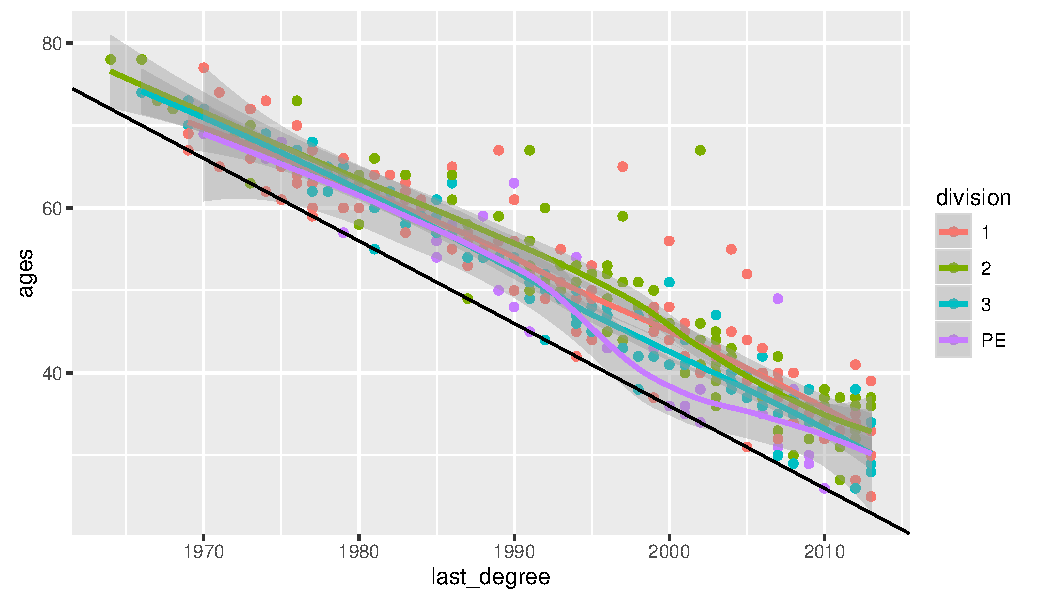
\includegraphics[width=\maxwidth]{figure/unnamed-chunk-7-1} \caption[Age with the year the last degree was received]{Age with the year the last degree was received}\label{fig:unnamed-chunk-7}
\end{figure}


\end{knitrout}

Division II professors seem to require longer to receive their last degrees, while PE professors require
less than others. It is also interesting to note the professors who take a significant amount of time
after receiving the BA to receive their last degrees. This is presumably because they spent some time out
of academia before entering graduate school. Most of these professors are from Division I and Division II,
which may indicate the importance of a terminal degree in Division III even outside of academia.\\

The professors who only received a BA can also be examined. Most of these professors are PE professors or
are in Division I, although there are some from Division II and Division III. This also demonstrates how
terminal degrees may not be considered as important when becoming a professor in Division I. This contradicts
the hypothesis that professors are younger because they were not required terminal degrees, since Division II
and Division III professors were on average younger than Division I professors. Thus the age distribution
may not depend greatly on whether the professors obtained a terminal degree or not.

\section{Conclusion}
This paper investigated the average age of the Williams College faculty, and how it was affected by
factors such as departments and terminal degrees. The data showed that PE professors are the youngest,
while Division II and Division III seem to be younger on average than Division I also. This result was also
compared with whether each professor were required a terminal degree, but it was concluded that this did not
have a significant influence on the age distribution in each division.

\end{document}
